%!TEX root = ../main.tex
\chapter{Der Gestaltungsprozess}
%Einleitungstext
Nachdem nun die wichtigsten Informationen zusammengetragen und analysiert wurden, kann mit dem eigentlichen Design-Prozess begonnen werden. Zu diesem Zweck werden wie in der Lehrveranstaltung Mediendesign gefordert verschiedene Design-Ansätze verfolgt. Zu gegebenem Zeitpunkt wird einer dieser Ansätze von einer Jury ausgewählt. Im Anschluss wird ein Style-Guide zu diesem Design erstellt und Unterseiten werden abgeleitet. Der Letzte Schritt besteht letzlich aus Optimierungs-Arbeiten.

%Einleitungstext_Ende
\input{./docs/chapter_2_designansätze.tex}
\section{Logo Entwürfe}
\begin{figure} [tp]

\includegraphics[width=\textwidth]{./img/logo1.png}
\caption{Der erste Logo Entwurf}
\label{logo1}
\end{figure}
\begin{figure} [tp]

\includegraphics[width=\textwidth]{./img/logo2.png}
\caption{Der zweite Logo Entwurf}
\label{logo2}
\end{figure}
Nun muss für DigitalHome ein Logo gefunden werden. Der erste Entwurf entstand im Zuge des minimalistischen sowie des zeitgemäßen Comps. Der zweite Logoentwurf entstand im Zuge des innovativen Comps. Um die Qualität des Logos besser beurteilen zu können, wurde hier das ARMM-Modell zu Rate gezogen. Auf Grund des ARMM-Modells (Attention, Response, Memory, Meaning) ist die Aufgabe des DigitalHome Logos, die Digitalisierung des Hauses in einem einfachen Symbol festzuhalten, das Aufmerksamkeit erregt, eine passende Emotion hervorruft, gut zu merken ist und einen tieferen Sinn hat. Deshalb besteht das Logo aus einem abstrahierten Haus, dessen Fassade aus 1 und 0 besteht.

Aufmerksamkeit erregt das Logo durch das Haussymbol. Haussymbole suggerieren das „nach Hause“ Gehen („Home“ bei Websites, „Startseite“ in Webbrowsern) und wirken damit sofort vertraut auf den Nutzer. Der Nutzer fühlt sich wohl und reagiert mit Vertrauen gegenüber der Brand DigitalHome. Da Menschen sich im Wesentlichen Umrisse und simple Formen merken (Gestalten Theorie), wurde hier besonders auf Einfachheit des Logos, geringe Anzahl an visuellen Elementen geachtet. Dadurch wird auch die Bedeutungsdichte höher, da es in beiden Entwürfen zwei visuelle Objekte (Dach, Fassade) gegenüber zwei Bedeutungen gibt (Haus, Digitalisierung). Dieses 1:1 Verhältnis rechtfertigt die Elemente des Logos und zeigt, dass hier nicht unnötig viele Elemente ohne Hintergedanken verwendet wurden.

Der Schriftzug enthält den Font Electrolize, der technisch wirkt und daher für dieses Logo gut geeignet scheint. Auf Grund der Unifarbigkeit lassen sich die Logos auf jedem Hintergrund benutzen.


Die Entwürfe unterscheiden sich in der Umsetzung dieser Grundidee. Im ersten Entwurf (Abbildung \ref{logo1}) werden bewusst Ecken gezeigt, sie sollen dem Logo einen technisch seriösen Aspekt geben. Die geraden Linien wirken simpel und straight-forward. Das „Dach“ wurde bewusst mit der „Fassade“ verbunden, damit das Logo eine einheitliche Form bildet. Insgesamt wirkt das Logo sehr technisch und kantig.


Das zweite Logo (Abbildung \ref{logo2}) bietet runde Ecken, die das Logo runder, weicher erscheinen lassen. Dazu wird es durch einen Kreis eingerahmt, um dem Logo einen festgelegten Platz zuzuweisen. Dabei wird darauf geachtet, dass das „Dach“ von der „Fassade“ des Hauses visuell getrennt ist, da sonst die „1 0“ Symbolik nicht mehr zum Vorschein kommt. Außerdem wird hier eine Pfeilform sichtbar. Pfeile zeigen, dass etwas in einer bestimmten Richtung geschieht (z.B. Bewegung). Deshalb werden Pfeile mit Bewegung assoziiert (z.B. Vektoren). Wichtig ist dabei, in welche Richtung der Pfeil zeigt. Man kennt Pfeile vor allem aus Diagrammen und nimmt die Richtungen oben und rechts als positiv war, wobei ein Pfeil nach rechts eine Zeitveränderung suggeriert (z.B. fortlaufendes x bei Funktionen), während der Pfeil nach oben eher einen Wertzuwachs zeigt (z.B. Aktienkurse). Der Pfeil im Logo wertet das Logo dementsprechend auf und erhöht die bereits erwähnte Bedeutungsdichte.

\subsection{Fontwahl}
Für die Gestaltung des Schriftzuges gibt es hier zwei verschiedene Vorgehensweisen. Normalerweise werden Wörter durch Freiräume getrennt (Leerzeichen, Carriage Return). Dies ist hier jedoch nicht empfehlenswert, da eine Trennung der Wörter zur Bildung von zwei verschiedenen Elementen innerhalb des Logos führen würde. Es würde dann aus dem Trademark, dem Schriftzug und noch einem Schriftzug bestehen. Um das zu umgehen, werden die Wörter mit anderen visuellen Mitteln unterschieden. Aus Gründen der Lesbarkeit wird das Letterspacing nicht verändert.

Das erste Logo setzt auf eine einheitliche Schriftart und unterscheidet die Wörter „Digital“ und „Home“ durch verschiedene Farben. Dadurch entsteht ein Bruch mit der Idee der Unifarbigkeit, die einheitliche Font bringt jedoch Konsequenz in das Schriftbild des Logos.
Das zweite Logo bleibt unifarben und damit flexibel, während die Schrift sich ändert. Diese zweite Font ist „Raleway“, welche auch auf der Website verwendet wird. Trotz der Tatsache, dass es sich bei beiden Fonts um Sans-serif Typefaces handelt, lassen sich beide Wörter aufgrund der unterschiedlichen Font-weight gut erkennen. Das Logo bleibt farblich flexibel, während die dünne Raleway Font Modernität und Leichtigkeit vermittelt und sich mit der technischen Electrolize Font zur perfekten Repräsentation der DigitalHome Marke vereint.

\section{Der Innovative Comp}
Der erste Eindruck zählt. Und Eindruck macht ein innovatives Unternehmen wie DigitalHome nicht zuletzt durch entsprechende Innovationen.
Darauf wird hier gesetzt, weshalb bei der Website ein ungewöhnliches Konzept zum Einsatz kommt: horizontal Scrolling. Man findet es fast gar nicht auf anderen Websites, vor allem aus Rücksicht auf Desktopnutzer, die mit ihrer Maus meistens nur vertikal scrollen können. Das hat sich mit seit 2013 geändert, wo nun mehr als 50\% der Nutzer über Handhelds und Touchscreens auf das Internet zugreifen und außerdem das Touchpad durch Laptops weit verbreitet ist.
Die Startseite soll der erste Anlaufpunkt für Nutzer sein und soll daher eine kurze Produktübersicht enthalten. Trotz der Innovation wird hier auf das gewohnte
Prinzip gesetzt, Content in aneinander gereihten Blöcken auf einer scrollbaren Seite zu präsentieren.

	\subsection{Comprehensive Dummy}

Eine erste Zeichnung des Comps hält die Grundidee fest (siehe Abbildung \ref{inno_Comp1}). Auf dieser Basis wird der Comp schrittweise zu einem fertigen Entwurf entwickelt.

\begin{figure} [hp]
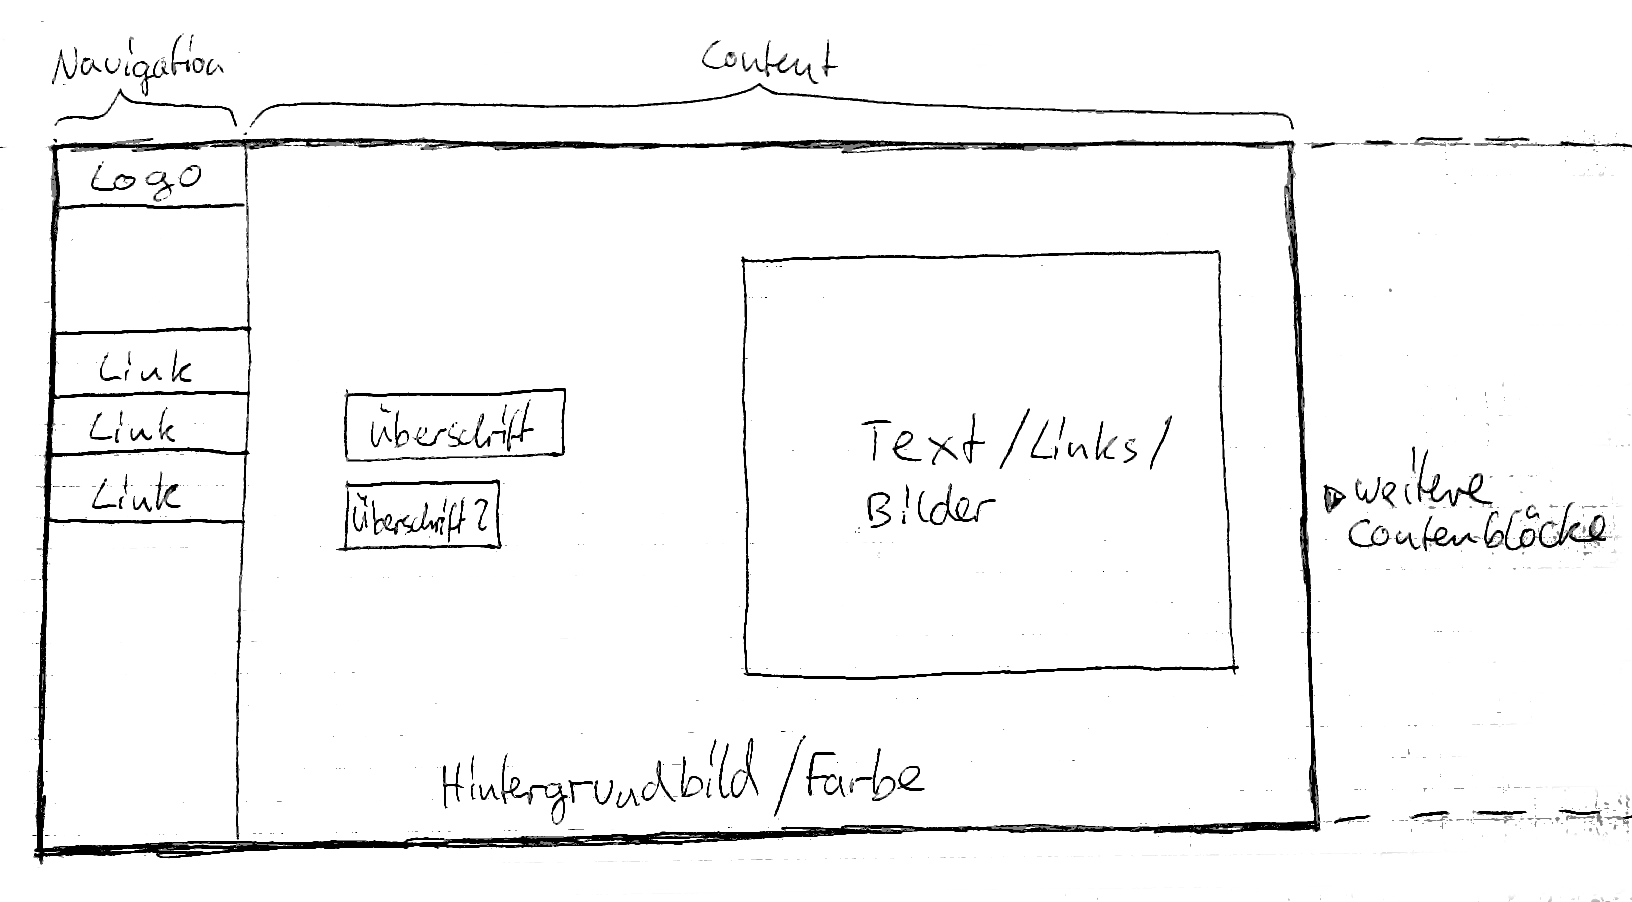
\includegraphics[width=\textwidth]{./img/inno_comp1.png}
\caption{Der erste Entwurf auf Papier}
\label{inno_Comp1}
\end{figure}
	\subsection{Entwicklungsphase HTML\&CSS}
\begin{figure} [tp]
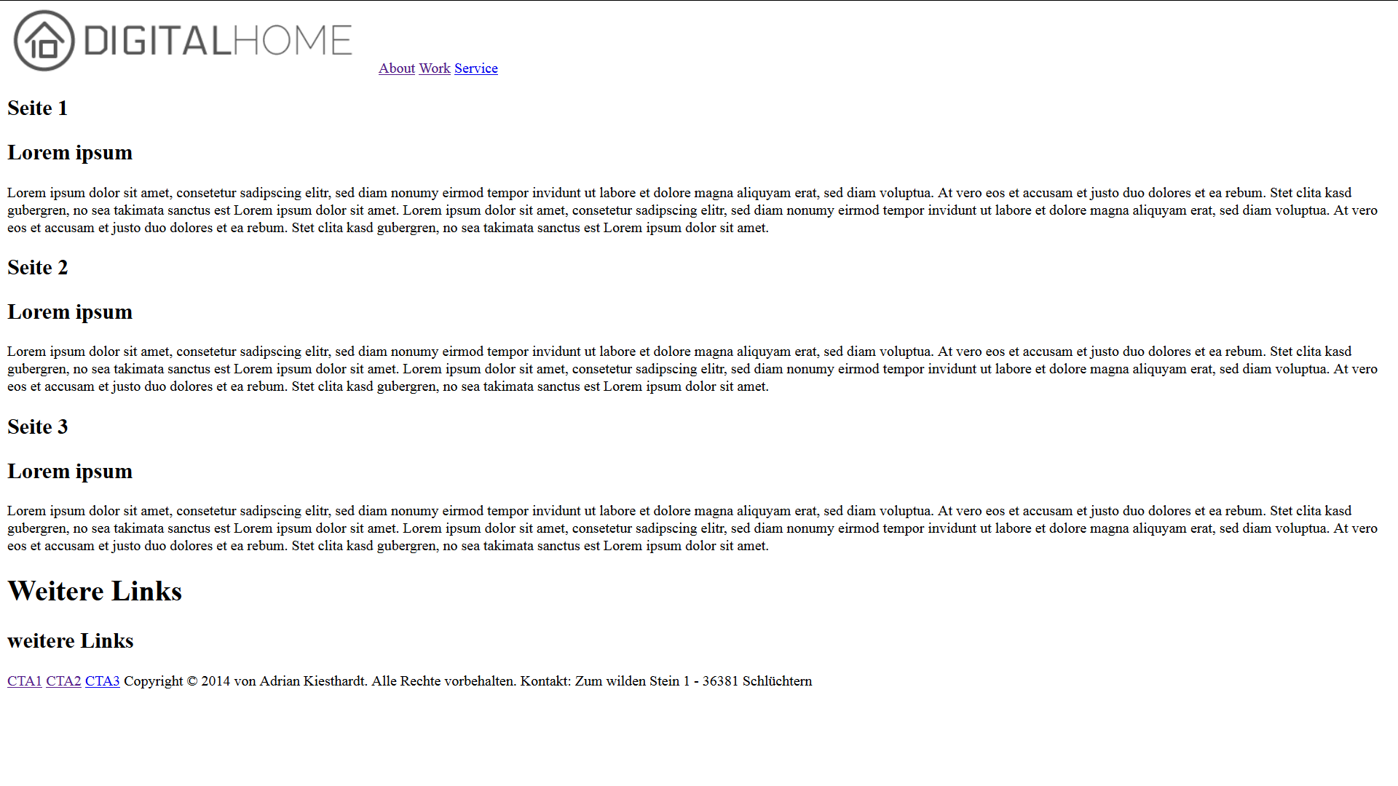
\includegraphics[width=\textwidth]{./img/inno_comp2.png}
\caption{Der erste Entwurf mit HTML}
\label{inno_Comp2}
\end{figure}
\begin{figure} [tp]
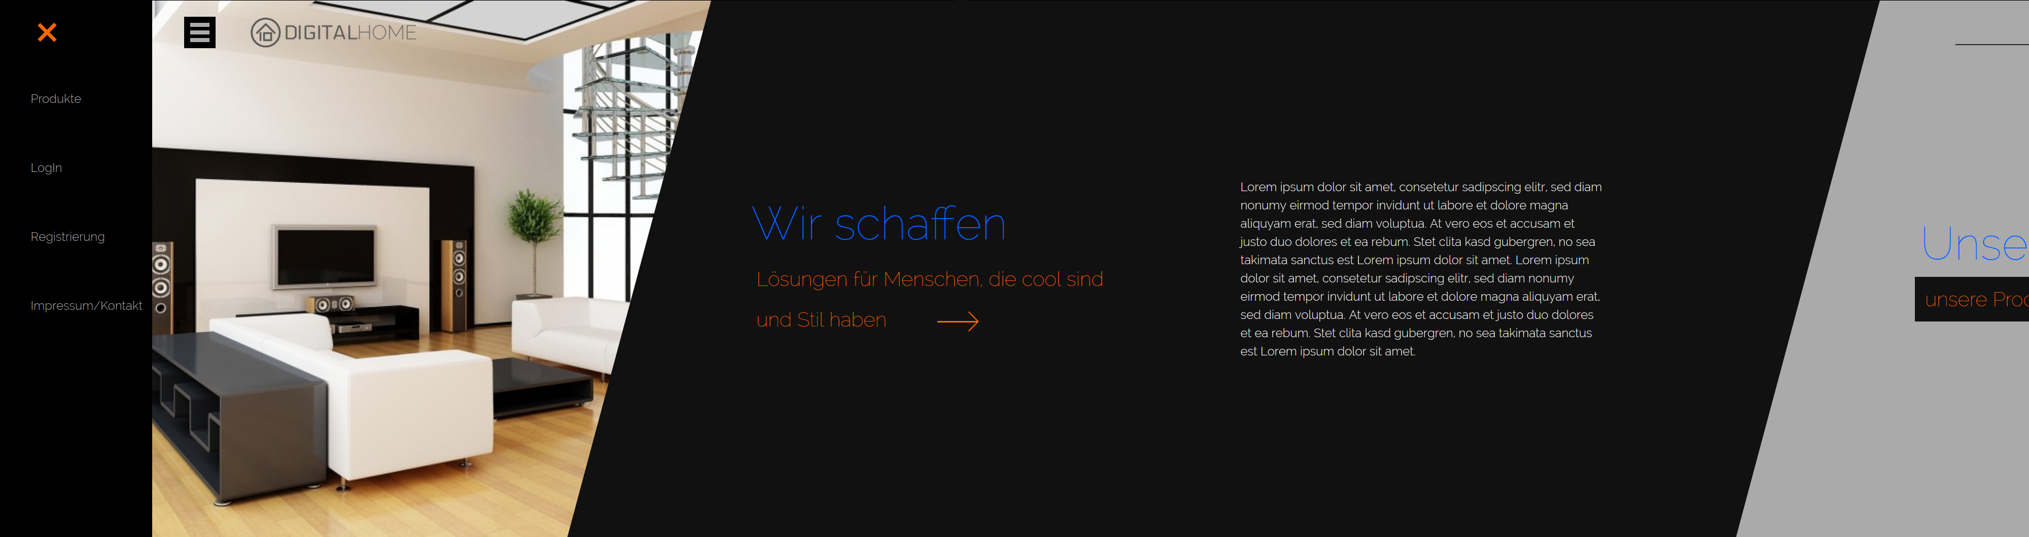
\includegraphics[width=\textwidth]{./img/inno_comp3.png}
\caption{Der erste Entwurf mit HTML\&CSS}
\label{inno_Comp3}
\end{figure}

Zur Umsetzung des horizontal Scrolling wäre es gut Tabellen zu verwenden, da diese die einzig sinnvolle Möglichkeit bieten, einen Container zu basteln, der sich abhängig vom Content nicht nach unten, sondern nach rechts erweitert (aufgrund der Eigenschaften von Tabellenzeilen). Da Tabellenlayouts mit <table> jedoch technisch hinter der Zeit, nicht responsive, unflexibel und semantisch falsch sind, braucht man eine Möglichkeit, das Tabellenlayout zu imitieren, ohne dabei Tabellen zu verwenden. Dazu werden in HTML die semantisch korrekten <section> Elemente verwendet (siehe Abbildung \ref{inno_Comp2}), die in CSS für das Tabellenlayout formatiert werden (siehe Abbildung \ref{inno_Comp3}). Die <section> Elemente werden als Tabellenzelle formatiert, die aufgrund der Organisation des <table> Elements in einer Zeile liegen. Der übergeordnete Container, der die Sections enthält, wird als Tabelle formatiert. Er breitet sich nach rechts aus und hat damit eine dynamische Breite. Die Sections haben jedoch eine relative Breite, die sich aufgrund des CSS bei Prozenteinheiten an dem übergeordneten Container orientieren würde, was nicht funktioniert. Die Container sollen ihre Größe an den Bildschirm anpassen, weshalb hier die Einheiten vw für „viewport width“ und vh für „viewport height“ eingesetzt werden.

	\subsection{Farbgebung\label{emo_col}}

Um der Innovation und Modernität gerecht zu werden, verwendet man Grautöne, hauptsächlich schwarz oder dunkle Grautöne. Da schwarz in enger Beziehung zum Tot steht, würde eine komplett schwarze Seite nicht einladend wirken. Wesentlicher eleganter wirkt Dunkelgrau. Schwarz lässt sich jedoch gut zur hierarchischen Abgrenzung spezieller Bereiche (z.B. Navigation) nutzen. Gleichzeitig muss ein Schwarzabgleich geschaffen werden, damit die Seite nicht zu hell wirkt und einen guten Kontrast bildet. Um diesen Kontrast nochmals zu unterstreichen, alterniert die Farbe des Hintergrunds. So entsteht ein Ausgleich zwischen dunklen und hellen Bereichen der Seite. Als Hintergrund wird also alternierend dunkelgrau/hellgrau, was seriös und einladend zugleich wirkt, und die Navigationsleiste wird schwarz. 

\begin{figure} [h]
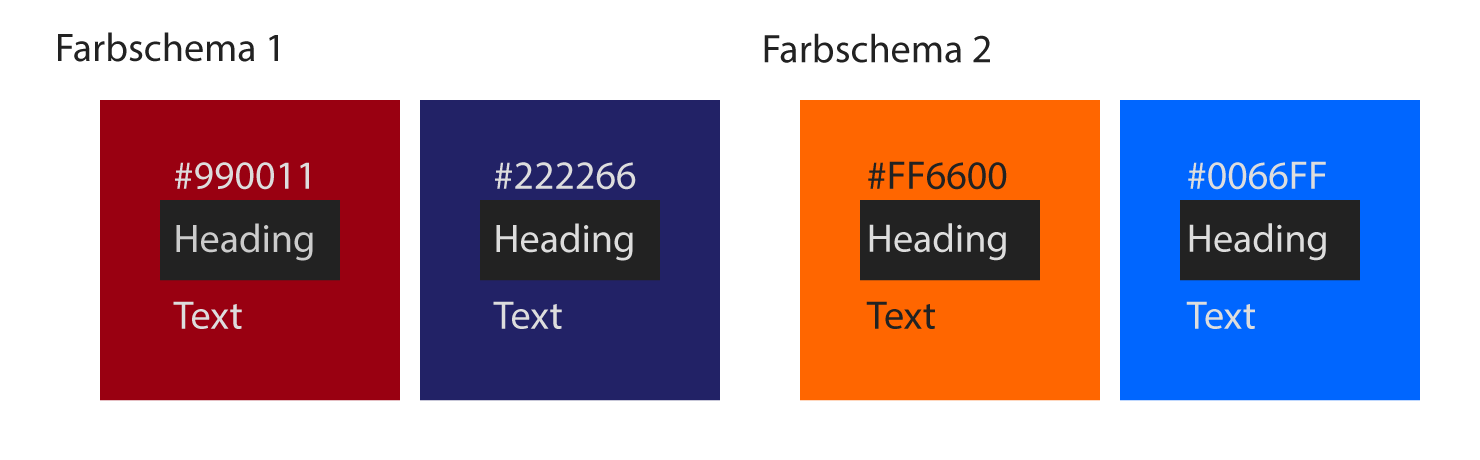
\includegraphics[width=\textwidth]{./img/inno_col1.png}
\caption{Diese Farbschemen kämen in Frage}
\label{inno_Farbschemen1}
\end{figure}


In grau wirkt die Seite ziemlich trist, deswegen kommen Akzentfarben zum Einsatz. Mehr als zwei Farbtöne sind zu bunt, ein einzelner Farbton belastet die Wirkung einseitig. Deshalb werden zwei Farben gewählt. Pastellfarben wirken seriös und edel, so kommt das erste Farbschema aus einem emotionalen rot und einem ruhigen, dunklen blau zu Stande. Das zweite Farbschema besteht aus stechenden Farben (siehe Abbildung \ref{inno_Farbschemen1}). Das wirkt künstlerisch, dynamisch, modern und kreativ. Orange ist zudem die Farbe der Kreativität. Als Ausgleich wird hier Himmelblau eingesetzt, das durch die direkte Assoziation mit dem Himmel Freiraum und Großzügigkeit vermittelt, aber auch kühl, technisch wirkt. In den zwei Farbschemen stehen sich ein warmer Farbton und ein kalter Farbton in ungefähr gleicher Helligkeit und Sättigung gegenüber, wodurch eine kontrastreiche und dennoch ausgeglichene ruhige, unaufdringliche Atmosphäre entsteht.

\begin{figure} [h]
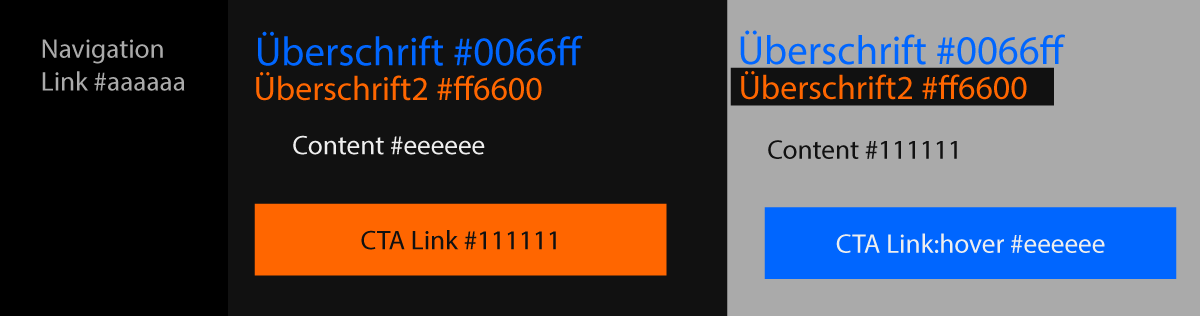
\includegraphics[width=\textwidth]{./img/inno_col2.png}
\caption{Das zweite Farbschema}
\label{inno_Farbschemen2}
\end{figure}

Der Grund, sich für das zweite Farbschema zu entscheiden, liegt darin, dass sowohl das erste als auch das zweite den Farbverlauf des Himmels gegen Abend wiederspiegeln. Das bindet den Menschen im Allgemeinen emotional, viele empfinden den Sonnenuntergang als romantisch. Das erste Farbschema drückt dieses Gefühl in einer sehr ruhigen Weise aus, stellt jedoch auf Grund der fehlenden Sättigung eher den Teil des Abends da, wenn die Sonne bereits untergegangen ist. Am stärksten ist das Gefühl zu jenem Zeitpunkt, an dem sich der Himmel blau orange färbt, wie im zweiten Farbschema. Dazu kommt, dass blau, orange auf dunklem Hintergrund besser zu lesen sind als dunkel rot, dunkel blau und das Menschen mit Rot-Grün-Schwäche orange im Gegensatz zu dunkel rot erkennen können. Daher wird hier das 2.Farbschema als Hauptfarbschema gewählt (siehe Abbildung \ref{inno_Farbschemen2}).
Ein bleibendes Problem ist der weiße Text auf schwarzem Hintergrund, der die Augen mehr belastet als schwarzer Text auf weißem Hintergrund. Jedoch bietet sich dunkler Hintergrund bei bildlastigen Seiten an wegen des Fehlens von störenden weißen Rändern um Bildern. Außerdem relativiert sich das Problem durch die geringe Textmenge und die alternierende Hintergrundfarbe.


	\subsection{Typographische Gestaltung}

Die Qualität des Designs wird vor allem durch das Zusammenspiel der einzelnen Faktoren bestimmt. Zu dem Layout und den Farben muss auch die Typografie passen. Dazu wurden Typefaces gesucht, die zum modernen und kreativen Auftreten von Digital Home und damit der Website passen. Da dem Projekt zurzeit keine kommerziellen Fonts zur Verfügung stehen, musste die Suche auf frei zugängliche Schriftarten beschränkt werden. Unter Rücksicht auf die Ladezeiten der Website und das Cachen der Fonts wurde hier Google Fonts als CDN für die gesuchten Typefaces gewählt.
Da die gesuchte Schriftart innovativ und technisch wirken soll, kann die Suche auf Sans-serifs beschränkt werden. Außerdem sollen durch dünne Linien Minimalismus und Reinheit betont werden. Unter jenen Sans-serif Schriftarten findet sich Raleway, welches sich selbst als Humanist-Sans bezeichnet. Dieser Teil der Font-Familie (Raleway Light bzw. Thin) hat jedoch auch stilistische Eigenschaften einer Geometric-Sans Font, welche in Architektur und Wissenschaft \footcite[vgl.][]{codeschool:typo} sehr beliebt sind. Zwischen diesen beiden Typen liegen die Transitional-Sans. Diese sind gut mit den Themen Technologie und Wirtschaft zu verbinden. Architektur und Technologie sind eben jene zwei Kernbereiche der DigitalHome Idee, weshalb sich diese Font letztlich so gut eignet.
        \begin{figure} [htp]
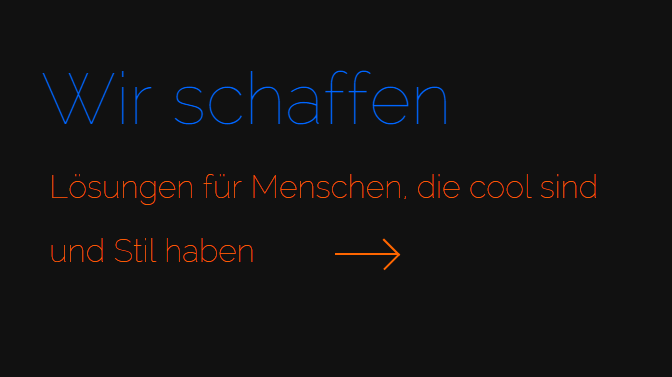
\includegraphics[width=\textwidth]{./img/inno_typo1.png}
\caption{Unterüberschrift mit Fontdicke 100}
\label{inno_Typo1}
\end{figure}

        \begin{figure} [htp]

\includegraphics[width=\textwidth]{./img/inno_typo1_2.png}
\caption{Bei der Dicke 100 treten unangenehme Effekte auf, weil sich Linien teilweise zwischen Pixel bewegen. Durch die Kantenglättung entstehen dann ungleichmäßig dicke Linien bzw. Punkte (Im Bild weiß makiert)}
\label{inno_Typo12}
\end{figure}

\begin{figure} [htp]
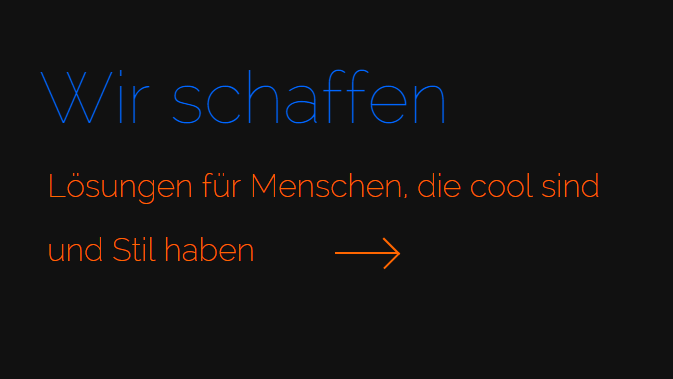
\includegraphics[width=\textwidth]{./img/inno_typo2.png}
\caption{Unterüberschrift mit Fontdicke 200}
\label{inno_Typo2}
\end{figure}
Das Ziel, eine möglichst dünne Font zu verwendet, muss aus Gründen der Lesbarkeit eingeschränkt werden. Während die Fontdicke 100 bei Überschriften gut funktioniert (siehe Abbildung \ref{inno_Typo1}), treten bei den Unterüberschriften unangenehme visuelle Effekte auf (siehe Abbildung \ref{inno_Typo12}), weshalb hier die Dicke auf 200 gesetzt wurde (siehe Abbildung \ref{inno_Typo2}). Textblöcke mit noch kleinerer Schrift bekommen die Dicke 300.


	\subsection{Strukturanalyse der Seite}

Da das Augenmerk beim Webdesign trotz der ungewöhnlichen Idee trotzdem auf Usability liegt, sollte das Wichtigste oben links stehen, nämlich wo der Nutzer sich befindet und wie er weiterkommt. Deshalb wird der Menubutton und das Logo in die linke obere Ecke verschoben. Beim Klick auf den Menubutton wird das Menu, welches OffCanvas und auch links liegt, von links eingefahren. Dadurch wird der Bezug zwischen dem Button und dem Menu selber hergestellt und Konsistenz wird gewahrt \footcite[vgl.][]{MaterialD:menu}.
 \begin{figure} [htp]
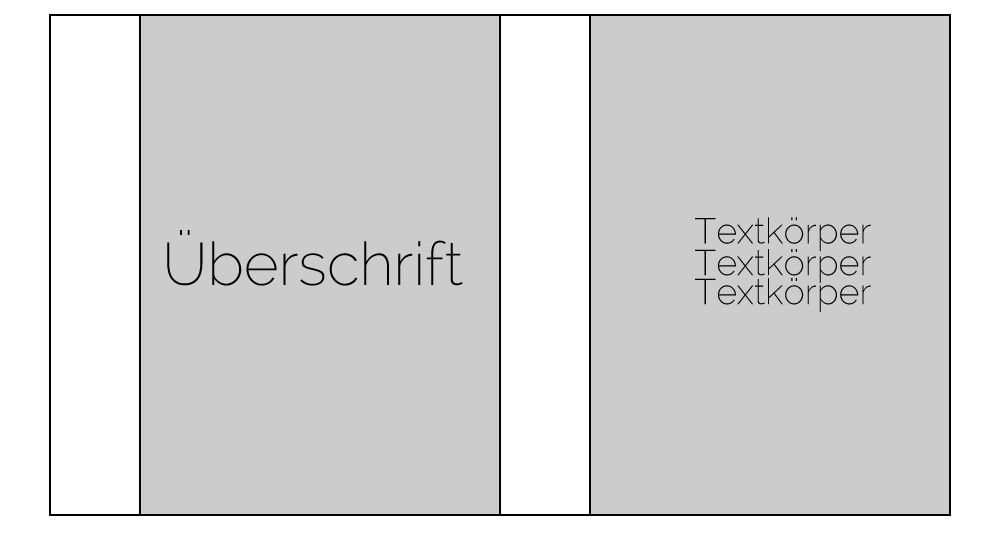
\includegraphics[width=\textwidth]{./img/inno_struct1.png}
\caption{zweispaltiges Layout}
\label{inno_Struct1}
\end{figure}
Das wichtigste an der Website ist der Content, in diesem Falle sind das Text und Bilder, die sehr sparsam eingesetzt werden. Deshalb kommt hier viel Whitespace zum Einsatz. Um den Content zu strukturieren, wird der einzelne Contentblock in der Mitte geteilt (siehe Abbildung \ref{inno_Struct1}). In dieser Halben „Seite“ kann ein Bild, eine Überschrift oder Text stehen. Der Content wird vertikal zentriert, damit sich der Whitespace gleichmäßig verteilt.

Stellt man die Sections als rechteckige Container dar, so wirkt die Kante zwischen den Sections beim Scrollen wie eine abrupt auftauchende Wand, die den Beginn eines neuen Abschnittes ankündigt. Deshalb kommen schräge Linien zum Einsatz, um das Design ein aufzubrechen [Inspiration: Dekonstruktivismus in der Architektur] und kommende Sections sanft einzuleiten. Hier soll damit vor allem erreicht werden, dem Design trotz seines simplen Aufbaus etwas Komplexes zu geben, damit es nicht langweilig wirkt und der Nutzer durch den entstehenden Überraschungseffekt länger an der Stange gehalten wird. Nach Tests im Bezug auf die Innen-und Außenabstände der Sections wurde sich hier auf eine $15\,^{\circ}{\rm}$ Neigung im Uhrzeigersinn geeinigt. Durch die dennoch gradlinigen Kanten bekommt die Seite einen Look, der gut mit der klinischen Atmosphäre der Farben harmoniert. 


Auf jeder Seite der Website soll als erstes ein Titelbild sein, um dem Nutzer schnell das Thema der Seite zu erklären. Redundant befindet sich auf der rechten Seite eine Überschrift, damit der Nutzer sichergehen kann, dass er sich auf der richtigen Seite befindet. Das sind die einzigen Bereiche, die above the fold liegen. Zusätzlich ist die Überschrift von reichlich Whitespace umgeben, damit sich der Nutzer nicht ablenken lässt. Beim weiterscrollen schließt sich direkt der restliche Content an.
Aufgrund der Preise der Produkte sowie der Seriosität, die über die Seite vermittelt werden soll, wird auf Werbung verzichtet. Außerdem werden auf der Startseite keine Preisschilder angezeigt, um nicht aufdringlich zu wirken.

Probleme dieses Designs zeigen sich in den schrägen Elementen Im Produkt Abschnitt. Die schrägen Links haben auf Grund von Kantenglättungsschwierigkeiten einen weißen Rand (Rendering), der hier durch einen 1px dicken schwarzen Rand (CSS) unterbunden wurde. Außerdem ist das Layout ziemlich unflexibel, da die Breite der Seite von der Anzahl der Elemente abhängen sollte, sich jedoch nicht dynamisch anpassen kann und daher separat geändert werden muss. Das bedeutet unnötigen Wartungsaufwand, der sehr schnell zu Schwierigkeiten (z.B. Bugs, Inkonsistenzen) führen kann.
Punkten kann dieser Entwurf jedoch mit seiner aufgeräumten Struktur, dem sehr innovativen Menübutton und dem ungewohnten Scrollverhalten

%!TEX root = ../main.tex
\section{Zeitgemäß}
Der Zeitgemäße Design-Entwurf hat zur Aufgabe dem Benutzer eine möglichst bekannte Nutzererfahrung zu bieten. Er soll sich direkt über bekannte Design-Elemente auf der Seite zurechtfinden. 
Jeder Designentwurf in diesem Ansatz verfolgt gleichzeitig den Ansatz des Mobile-First. Demzufolge werden verschiedene Endgeräte in die Überlegungen mit einbezogen.

\subsection{Comprehensive Dummy}
\begin{figure} [hp]
	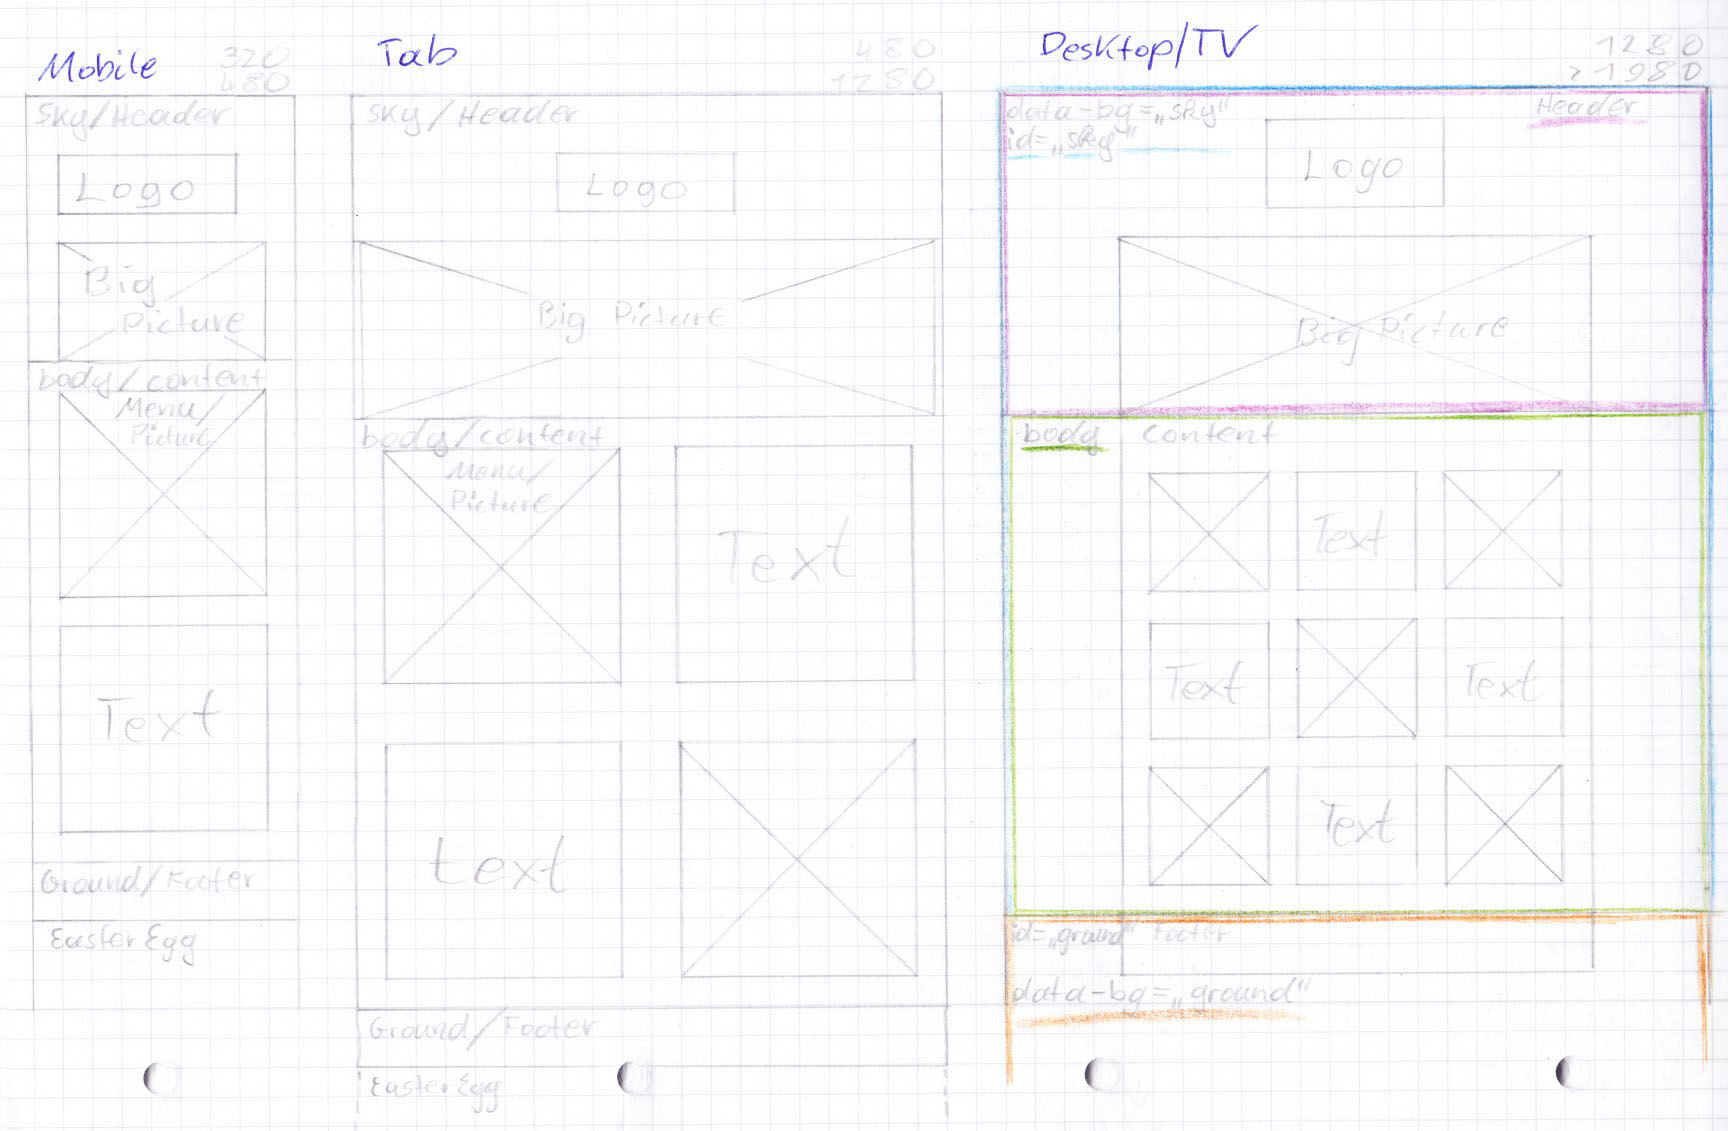
\includegraphics[width=\textwidth]{./img/zeitg_comp1.jpg}
	\caption{Ein erster Entwurf des zeitgemäßen Ansatzes mit Stift und Papier.}
	\label{zeitg:Comp1}
\end{figure}

Die erste Version des Comprehensive Dummy setzt ein Kacheldesign für Inhalts- und Bildblöcke in Form von Fenstern eines Hochhauses um. Wie in Abbildung \ref{zeitg:Comp1} zu sehen ist, wird hier auf ein bekanntes vertikales Layout bestehend aus den drei großen Bereichen, Kopf, Köper und Fußzeile vertraut. In der Kopfzeile soll ein großes Bild die Aufmerksamkeit des Users fangen. Neben dem Logo und einem Himmel als Hintergrund wird ansonsten auf weitere Inhalte im Header verzichtet. Auf mobilen Endgeräten wird noch auf ein einspaltiges Layout gesetzt, welches auf größeren Geräten mehr Spalten erhält um den Platz effektiv zu nutzen. Als designtechnisches Element wird auf Bildschirmen mit genügend Platz ein Whitespace mit Hintergrundgrafik links und rechts der Inhaltsblöcke verwendet.

Nach weiteren Überlegungen entsteht ein weiterer Comprehensive Dummy. Die Entscheidung zu diesem Schritt fußt auf den Überlegungen, dass zum einen eine Navigation in bekannter Weise fehlt und zum anderen das Bild eines Hochhauses nicht zur Zielgruppe der privaten Hauseigentümer passt.
Abbildung \ref{zeitg:Comp2} zeigt einen Ansatz, bei dem sich das Design am Logo orientiert. Auch hier stellt es im Grunde eine abstraktion eines Hauses dar. Diesmal jedoch ist ein Menü direkt am oberen Ende präsent. Ebenso sind die Inhaltsblöcke wieder als Fenster angedeutet.

\begin{figure} [hp]
	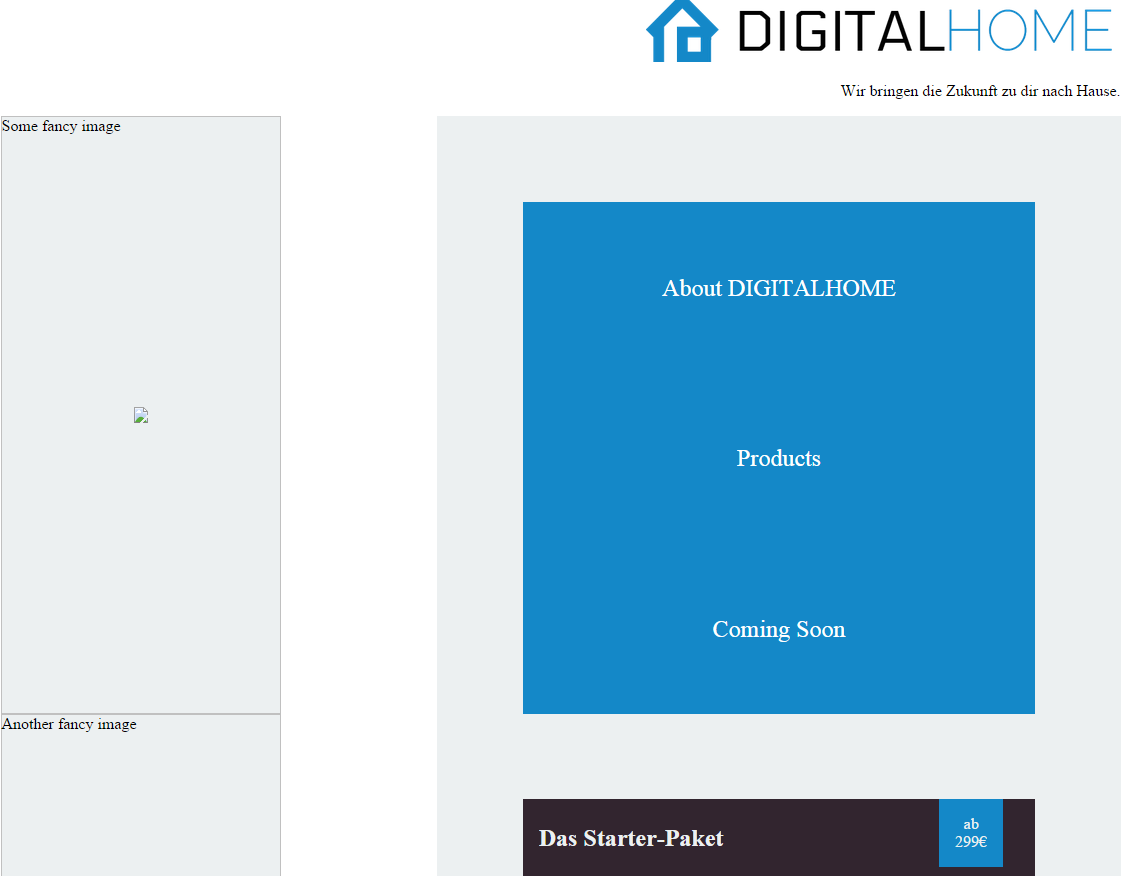
\includegraphics[width=\textwidth]{./img/zeitg_comp2.png}
	\caption{Der zweite Entwurf des zeitgemäßen Ansatzes. Diesmal bereits in HTML und CSS.}
	\label{zeitg:Comp2}
\end{figure}

Letzten Endes ist auch dieses Design nicht vertraut genug und etwas zu minimalistisch. Es folgt der letzte Entwurf, der explizit bekanntere Wege geht (siehe Abbildung \ref{zeitg:Comp3}. Weitere Einzelheiten zur Analyse der Struktur folgt im Kapitel \nameref{zeitg:struktur} auf Seite \pageref{zeitg:struktur}.

\begin{figure} [hp]
	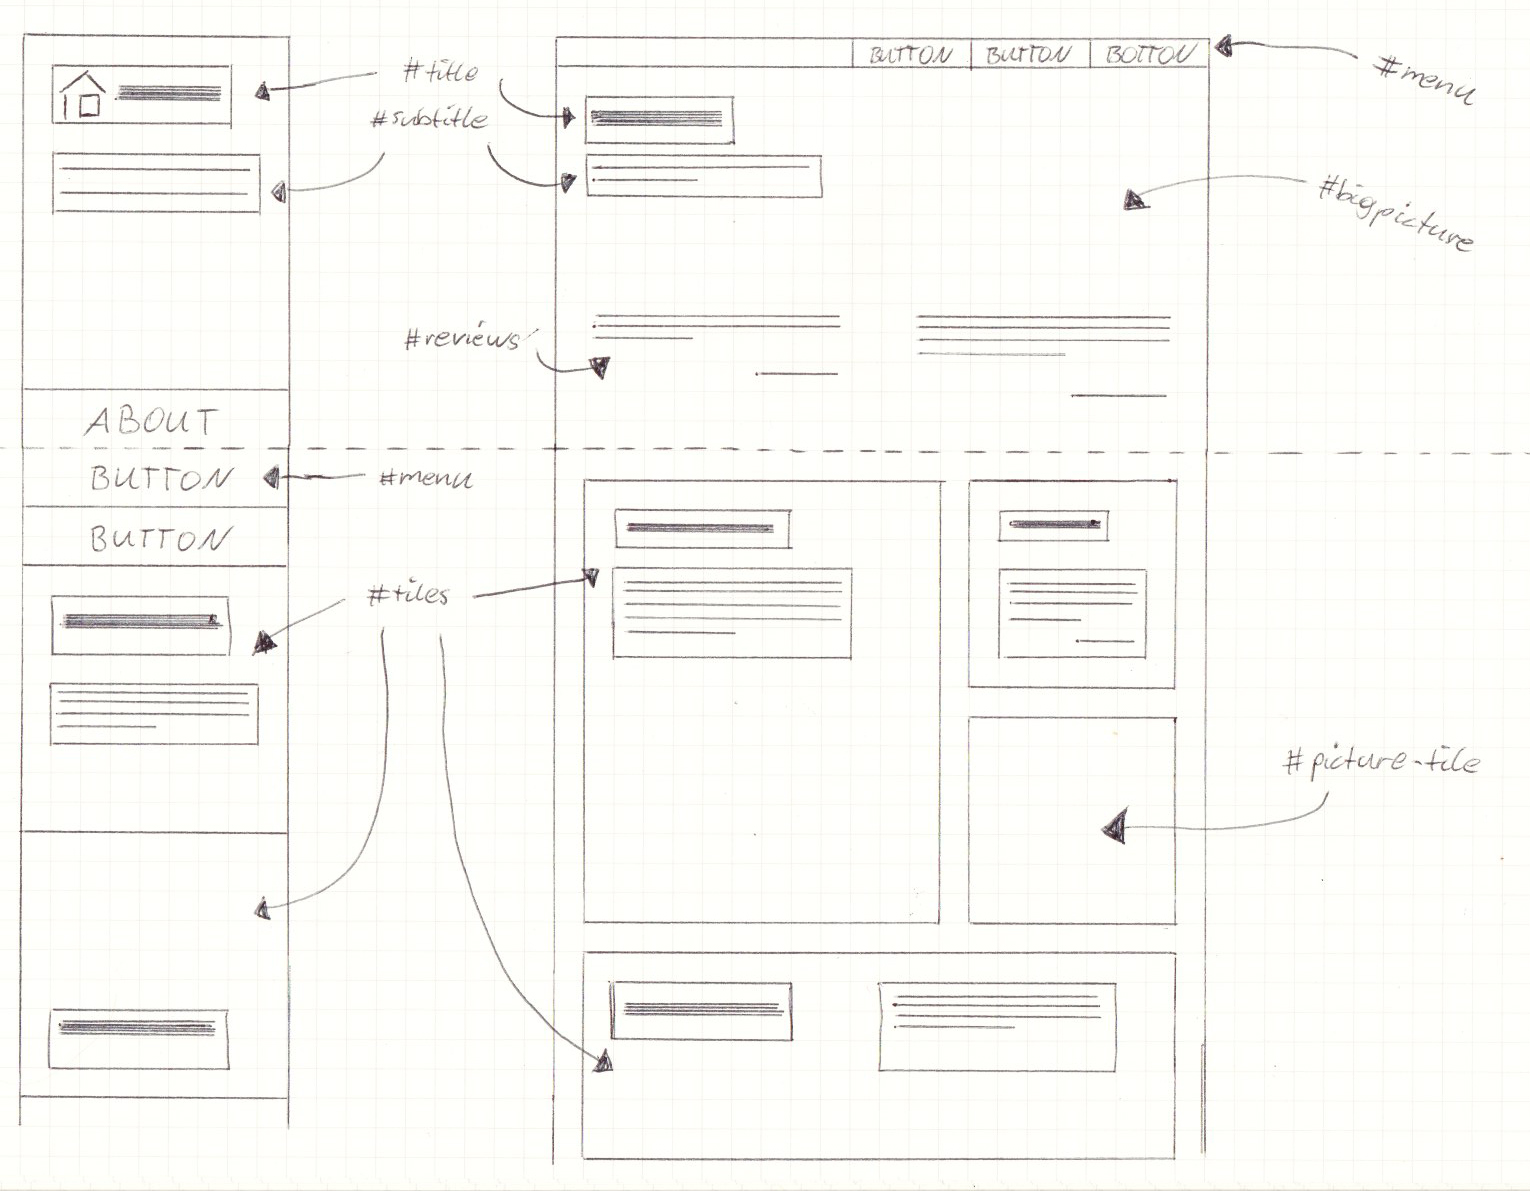
\includegraphics[width=\textwidth]{./img/zeitg_comp3.jpg}
	\caption{Der dritte und letzte Entwurf des zeitgemäßen Ansatzes mit Stift und Papier}
	\label{zeitg:Comp3}
\end{figure}

\subsection{Entwicklungsphase HTML\&CSS}
Die Entwicklung des Markups in HTML stützt sich auf das neue HTML5 und nutzt somit HTML-Tags wie \lstinline{<section>}, \lstinline{<nav>} und \lstinline{<footer>}.
Interessant bzw. speziell ist in diesem Zusammenhang lediglich noch das verwendete Kachel-System, welches eigens für diese Seite entwickelt wurde. Hierbei wurde auf die sog. AM-Modules zurückgegriffen.\footcite[vgl.][]{glen:am} Bei diesem Ansatz definiert man statt CSS-Klassen CSS-Attribute und weißt ihnen die Styles zu. Der Vorteil liegt hierbei im Namespace-Charakter. Der Namespace für die Kacheln lautet \lstinline{[am-Tile]}. Im Codeauszug \ref{code:zeitg:css1} ist zusehen, wie dem Namespace zuerst ein Grundstil vergeben wird und anschließend auf Elemente mit der Eigenschaft \lstinline{~="featured"} weitere Verfeinerungen angewendet werden.

\begin{lstlisting}[caption=AM-Modules zur Definition eines Namespace in CSS., label=code:zeitg:css1]
[am-Tile] {
	width: $column-width;
	padding-bottom: $column-width;
	position: relative;
	margin-bottom: $column-margin;
	margin-left: $column-margin;
	transition: all .3s linear;
	float: left;
}
[am-Tile~="featured"] {
	padding-bottom: 2 * $column-width + $column-margin;
	width: 2 * $column-width + $column-margin;
}
\end{lstlisting}

Desweiteren wird der CSS Code in der Präprozessor-Sprache SCSS geschrieben und anschließend in Valides CSS compiliert. Zu sehen anhand des Codeauszugs \ref{code:zeitg:css2}.

\begin{lstlisting}[caption=Verschachtelung von CSS-Klassen in SCSS., label=code:zeitg:css2]
nav {
	flex-direction: row;
	justify-content: flex-end;
	flex-flow: row wrap;
	& > a {
		padding: 0 2.5em;
		flex: 0 0 auto;
	}
}
\end{lstlisting}

\subsection{Farbgebung}
\begin{figure} [hp]
	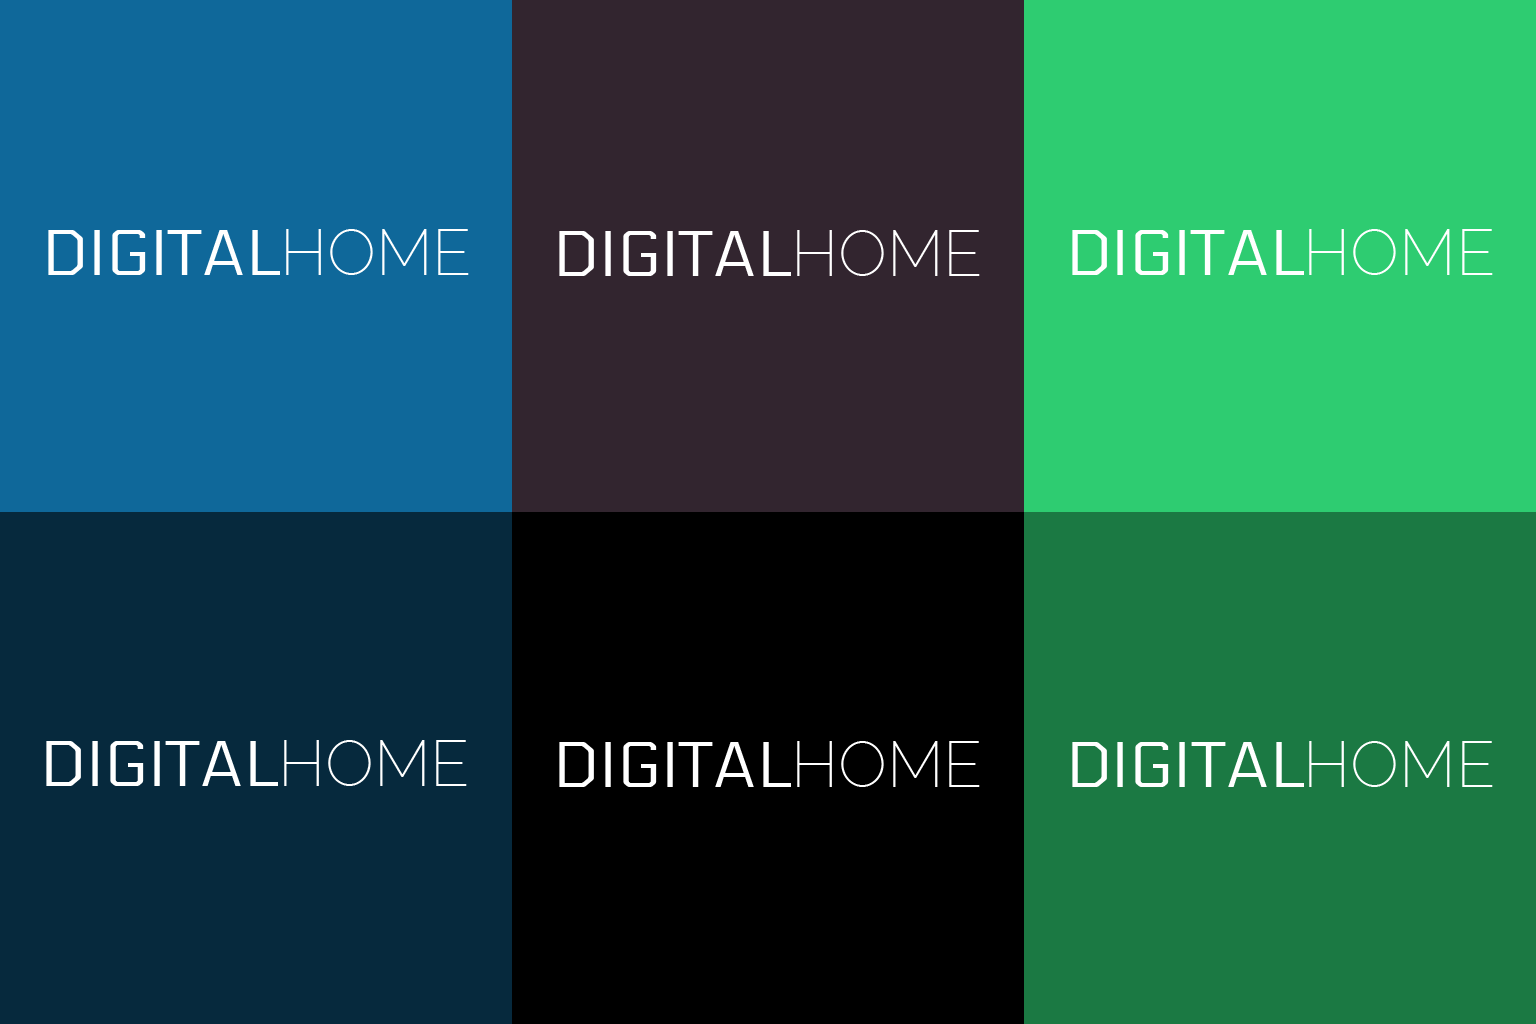
\includegraphics[width=\textwidth]{./img/zeitg_farbschema1.png}
	\caption{Das Farbschema des zeitgemäßen Ansatzes.}
	\label{zeitg:farbschema}
\end{figure}

Für den zeitgemäßen Ansatz wurde auf ein Monochromatisches Farbschema gesetzt, wie in Abbildung \ref{zeitg:farbschema} zu sehen. Blau und Schwarz sind Hauptfarben des Designs, Grün dient als alternative zu Blau.
Blau kommt aufgrund seiner Assoziation mit Technik und Intelligenz zum Einsatz. Die Farbe soll bei den Nutzern Vertrauen zur Seriösität des Unternehmens herstellen. Der Einsatz eines simplen Farbschemas ist vor allem der Bildlastigkeit des Designs zu verschulden.
Alle Farben sind als Pastellfarben auf eine gute Lesbarkeit ausgelegt. Ebenso wird die Webseite dadurch ruhiger und wirkt weniger Aufdringlich. Der Stresslevel wird reduziert.
Das alternative Farbschema ist ein völlig anderer Ansatz und soll trotz des technischen Konzepts ein Bezug zur Natur hergestellt werden. Der Nutzer soll hiermit eine Natürlichkeit bzw. Selbstverständlichkeit der Digitalisierung als Teil der Natur assoziieren.

\subsection{Typographische Gestaltung}
Für Überschriften und Texte wird ausschließlich auf die Font Familie Raleway zurückgegriffen. Aus dieser Familie kommen die Schriftbreiten 100 - 300 zum Einsatz, die unter Light/Thin geführt werden. Raleway bezeichnet sich selbst als Humanist-Sans. Dieser Teil der Font-Familie hat jedoch auch stilistische Eigenschaften einer Geometric-Sans Font, welche in Architektur und Wissenschaft sehr beliebt sind. Zwischen diesen beiden Typen liegen die Transitional-Sans. Diese sind gut mit den Themen Technologie und Wirtschaft zu verbinden. Architektur und Technologie sind eben jene zwei Kernbereiche der DigitalHome Idee, weshalb sich diese Font letzlich so gut eignet.
Auch in den anderen Ansätzen kommt diese Schriftart zum Einsatz. Vgl. Kapitel \ref{typo_inno} und \ref{chapter:mini:typo}.

\subsection{Strukturanalyse der Seite}\label{zeitg:struktur}
Strukturell ist dieser Ansatz recht konservativ mit einer Navigation am oberen Bildschirmrand, einem großen Blickfänger darunter und unter diesem der Inhaltsbereich im Kachel-Design. (Siehe Abbildungen \ref{zeitg:struktur1} und \ref{zeitg:struktur2})
Auf dem Blickfänger bzw. Titelbild ist das Logo mit dem Firmenname gut Sichtbar platziert, sowie eine Unterüberschrift direkt darunter. Zur besseren Lesbarkeit sind beide Blöcke durch Whitespace getrennt und haben einen Innenabstand von 1.5rem auf 16px normalisiert. Der Logo Block und die Unterüberschrift haben einen Abstand von 32px zueinander.

\begin{figure} [hp]
	
\includegraphics[width=\textwidth]{./img/zeitg_struktur1.png}
	\caption{Startseite im Programmierten Design. Navigation und Titelbild.}
	\label{zeitg:struktur1}
\end{figure}

\begin{figure} [hp]
	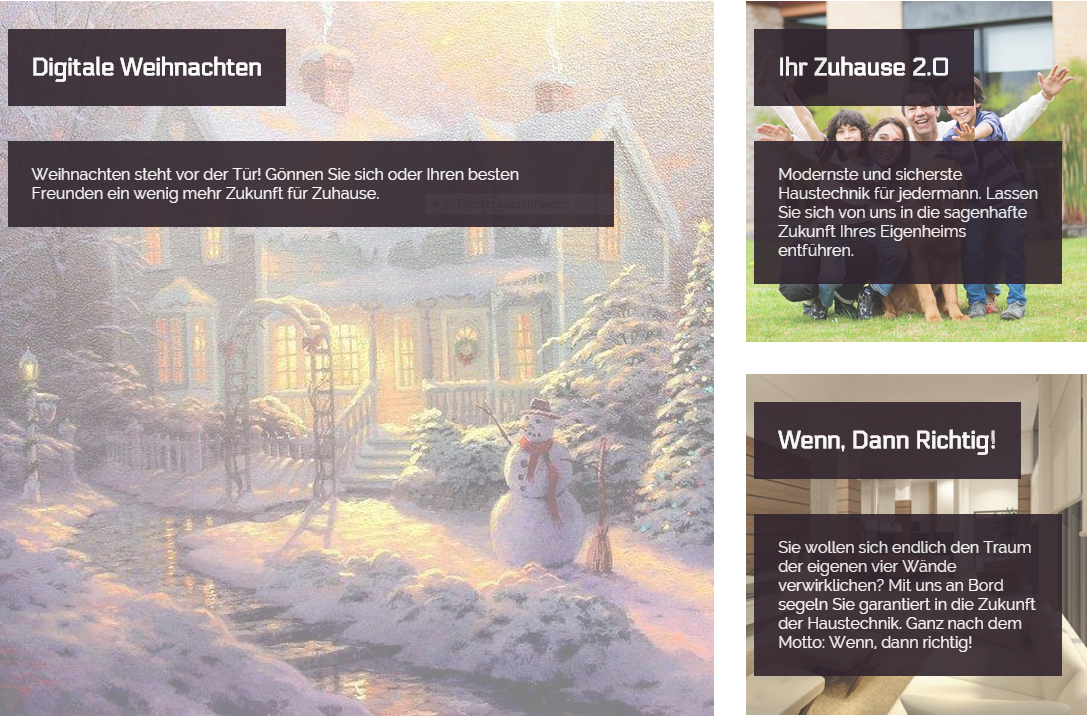
\includegraphics[width=\textwidth]{./img/zeitg_struktur2.png}
	\caption{Inhaltsbereich im programmierten Design des zeitgemäßen Ansatzes. Kacheldesign zum Darstellen des Inhalts.}
	\label{zeitg:struktur2}
\end{figure}

Um Botschaften zum Nutzer zu übertragen werden in diesem Design größtenteils Bilder verwendet, wie auch an dem großen Titelbild in Abbildung \ref{zeitg:struktur1} zu sehen ist. Transparenz der Schriftblöcke erleichtert das Erkennen der Bilder im Hintergrund. (Zu sehen in Abbildung \ref{zeitg:struktur2}).
Das Kachel-System in diesem Design basiert auf einem Grid-System mit einer Spaltenbreite von genau 320px und einem Spaltenabstand von 32px. Das System ist darüber hinaus mobil optimiert und folgt dem Responsive Webdesign Principle\footcite[vgl.][]{alistapart:rwd}. Anders als im allgemeinen Konsens arbeitet das System allerdings nach dem Adaptive Design Principle, welches ein bestandteil des RWD darstellt. Dabei gibt es CSS-Breakpoints für bestimmte definierte größen, wodurch das Design auch auf mobilen Geräten gut präsentiert wird. Wenn auch angemerkt werden muss, dass dieses Prinzip nicht derart flexibel ist wie ein Fluid-Design.
Zur besseren Hervorhebung und differenzierung einzelner Inhaltsblöcke gibt es verschiedene Arten von Kacheln. Standard sind hier die rechteckigen Kacheln der größe 320px. Kacheln mit der Eigenschaft \lstinline{~="featured"} werden in doppelter Größe in Höhe als auch Breite dargestellt. Die Eigenschaft \lstinline{~="extra"} verleiht der Kachel eine doppelte Breite.
Auf mobilen Endgeräten werden alle Kacheln auf Standardgröße reduziert sowie in einer einzigen Spalte angezeigt. Außerdem wird das Menü unter dem großen Bildbereich positioniert (Siehe Abbildung \ref{zeitg:struktur3}, derart, dass bei jeder Bildschirmgröße der Anfang des Menüs zu erkennen ist.

\begin{figure} [hp]
	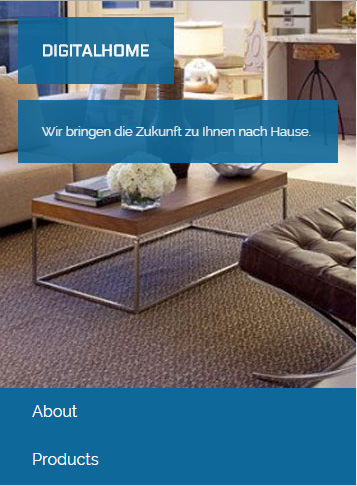
\includegraphics[width=0.5\textwidth]{./img/zeitg_struktur3.png}
	\caption{Startseite im Programmierten Design in der mobilen Ansicht. Navigation unter dem großen Bildbereich positioniert.}
	\label{zeitg:struktur3}
\end{figure}
\section{Minimalistisch}
Es gibt immer Webshops, wo die Seiten überladen sind mit eigentlich unnötigen Sachen oder Werbung. Als Idee hat dieser Webshop-Entwurf, dass die Seite minimalistisch gehalten wird, um so viel wie möglich auszudrücken bei minimalem Design.  
\\
Diese Seite ist durch Responsive Designing auch für Handhelds und Tablets geeignet.
	\subsection{Comprehensive Dummy}
Der zeichnerische Entwurf (siehe Abbildung \ref{mini_comp1}) zeigt schon, wie die Grundidee umgesetzt werden soll. So wurde dieser  
\begin{figure} [hp]
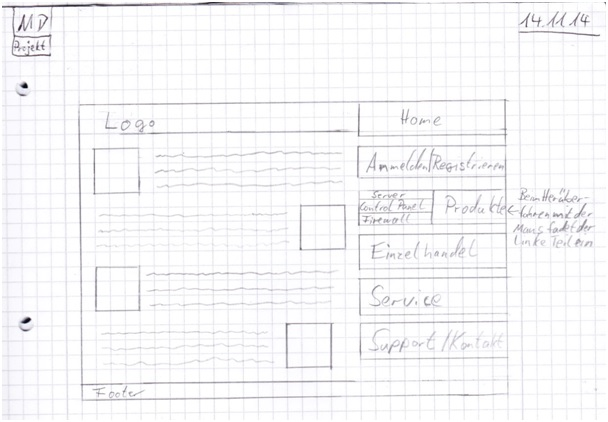
\includegraphics[width=\textwidth]{./img/mini_comp1.png}
\caption{Der Umsetzung der Idee auf Papier}
\label{mini_comp1}
\end{figure}
	\subsection{Entwicklungsphase HTML\&CSS}
Der erste Entwurf des Comps wurde in HTML umgesetzt. Hierbei sah man noch nicht viel von der Strukturierung, wie es im Comprehensive Dummy gedacht ist. Die Elemente waren einfach untereinander angeordnet. (siehe Abbildung  \ref{mini_comp2})
\\
\begin{figure} [hp]
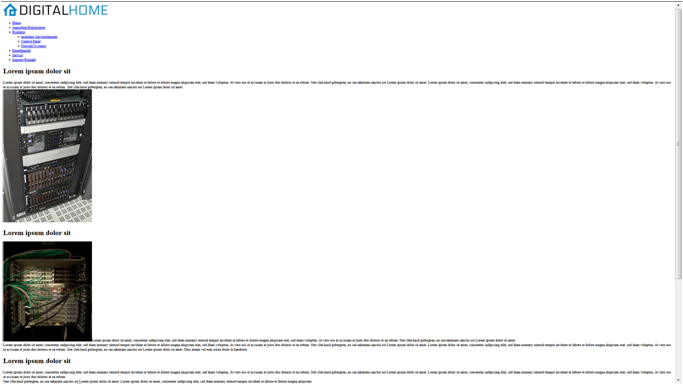
\includegraphics[width=\textwidth]{./img/mini_comp2.png}
\caption{Die erste Umsetzung in HTML}
\label{mini_comp2}
\end{figure}
Als dann zusätzlich noch CSS implementiert wurde, nahm die Seite ihre Form an, wie sie Comprehensive Dummy sein soll. Hierbei bereitete die Menüleiste Probleme, die anfangs noch manche Elemente überdeckt hat. Da Unterkategorien direkt bei den Navigationspunkten in der vorgesehenen Anordnung nicht funktioniert hat, wurde dies herausgenommen. Die Unterpunkte bekommt man stattdessen dann, wenn man auf den jeweiligen Navigationspunkt drückt im Content-Bereich angezeigt. Der Fehler, wo andere Elemente von der Navigationsleiste überdeckt werden, wurde durch Anpassen der Breiten und Höhen der Elemente beseitigt.
\\
Das Responsive Design bereitete auch Probleme. Dies wurde jedoch behoben, wodurch man, trotz des Entfernens der Unterkategorien, einen sehr originaltreuen Comprehensive Dummy als Webseitenentwurf hat. (siehe Abbildung  \ref{mini_comp3})
\begin{figure} [hp]
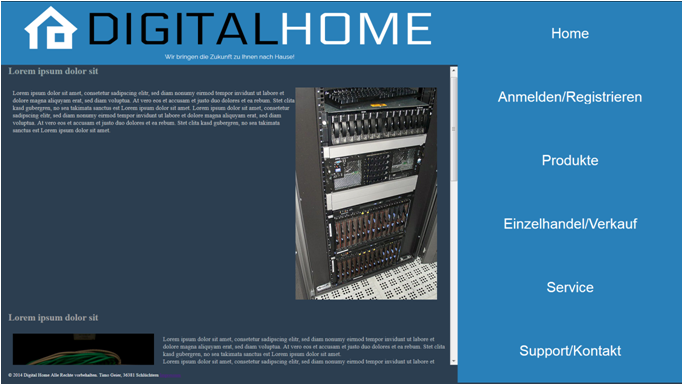
\includegraphics[width=\textwidth]{./img/mini_comp3.png}
\caption{Die endgültige Umsetzung mit HTML und CSS}
\label{mini_comp3}
\end{figure}

	\subsection{Farbgebung}
Da der Webshop Digitale Haustechnik verkauft, sollten die Farben offen und sehr intelligent wirken, zudem eine gewisse Ruhe und Kühle ausstrahlen. Aber es sollte auch zum Minimalismus des Seitenaufbaus passen.
\\
\\
Deswegen basiert das Farbschema in der Online-Fassung hauptsächlich auf blauen Farbtönen, wie man aus dem Bild sehen. Die Hintergrundfarbe und die Footerfarbe sind in einem dunklen Blau, das Ruhe, Konzentration und Sachlichkeit von Informationen symbolisiert. 
Sowohl der Header, als auch die Elemente der Navigationsleiste sind in unterschiedlichen Blautönen, je nachdem, ob man mit dem Cursor über den Header oder die Elemente der Navigationsleiste fährt oder nicht. Sie sollen offen und intelligent wirken. Zusätzlich sind diese Farben im Kontrast zum Hintergrund und Footer, wodurch sie sehr im Fokus stehen.
\\
Die Überschriften und die Texte sind in jeweils zwei unterschiedlichen Grautönen gefärbt. Diese sollen die Sachlichkeit, Funktionalität, Schlichtheit, und den Minimalismus der Seite ausdrücken. Zudem kann man die Absätze dadurch besser voneinander unterscheiden.
\\
Die Schriftfarbe des Footers ist weiß, damit man den sehr gut lesen, denn er enthält wichtige Informationen zum Copyright, dem Webseitenbetreiber und zudem den Link zum Impressum der Seite. (siehe Abbildung \ref{mini_farb1})
\begin{figure} [hp]
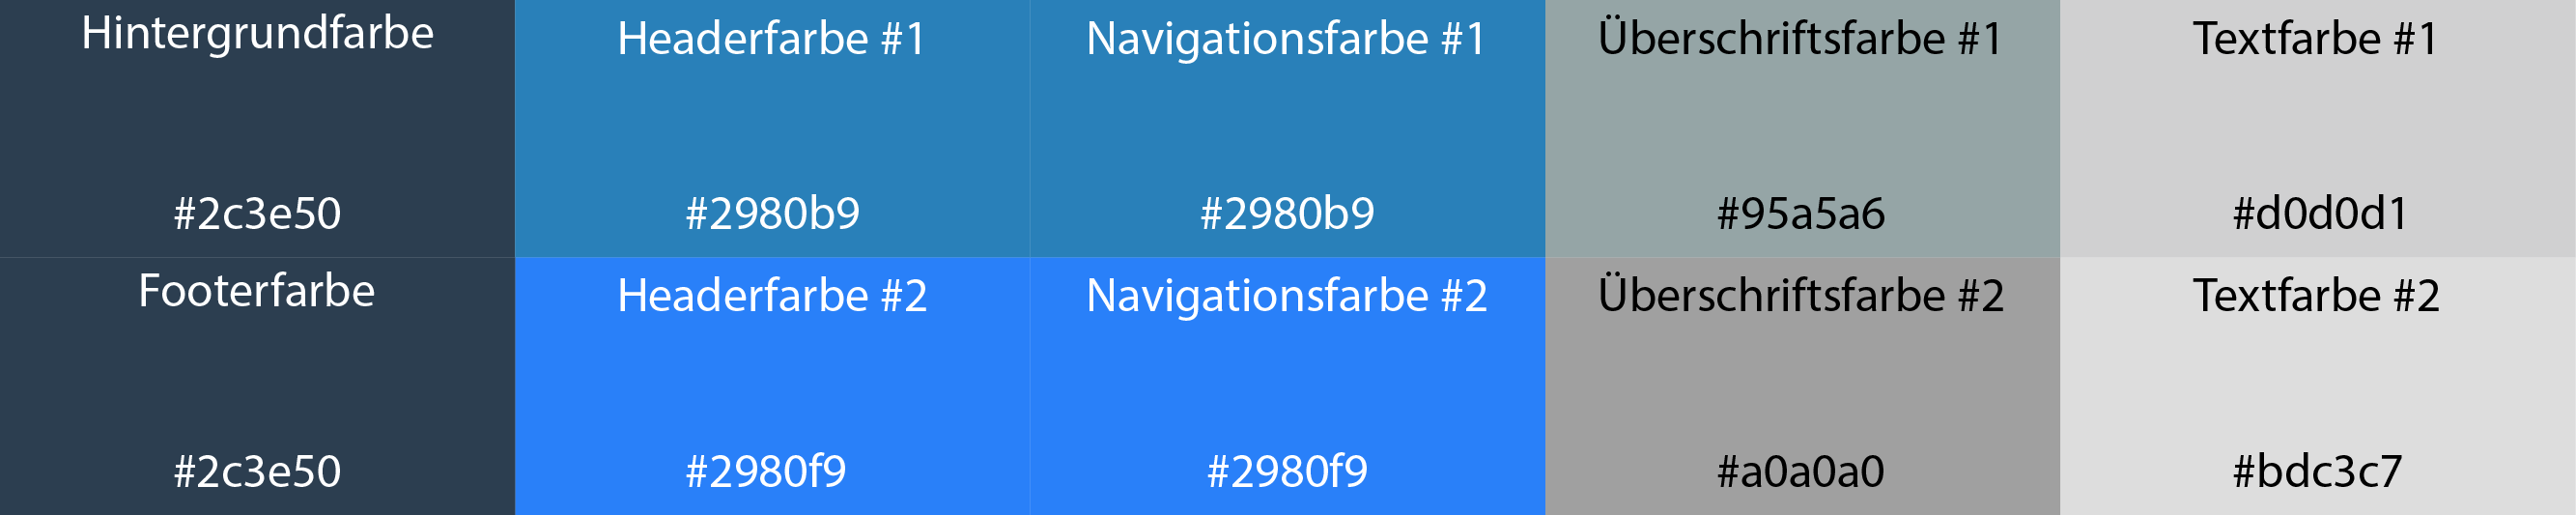
\includegraphics[width=\textwidth]{./img/mini_farb1.png}
\caption{Das Hauptfarbschema}
\label{mini_farb1}
\end{figure}

Als 1. alternatives Farbschema wurde ein geteilt komplementäres Farbschema gewählt. Dieses steht sehr zum Kontrast zum Hauptfarbschema. (siehe Abbildung \ref{mini_farb2}) 
\\
Die Hintergrundfarbe ist orange mit Gelbstich. Die ist positiv besetzt, und symbolisiert zudem Sonnenschein und Kreativität. Dadurch wirkt die ganze Shopseite auch ungezwungener, was bei der Vermarktung von Produkten auch wichtig ist. Zusätzlich vermittelt orange eine gute Wohnatmosphäre.
\\
Für den Header und die Navigationsleiste wird die Komplementärfarbe zu orange, blau, verwendet. Diese steht für Offenheit, Intelligenz und Vertrautheit. Dadurch passt es auch zu dem Angebot der digitalen Haustechnik. 
\\
Der Text ist in schwarz beziehungsweise dunklen Grautönen gehalten, und ist somit ein guter Kontrast zum Hintergrund. Zusätzlich drückt sie Eleganz und Stärke aus.

\begin{figure} [hp]
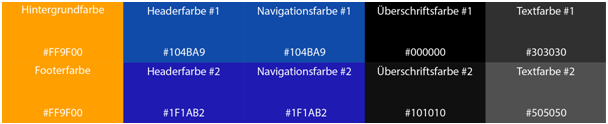
\includegraphics[width=\textwidth]{./img/mini_farb2.png}
\caption{Das 1. alternative Farbschema }
\label{mini_farb2}
\end{figure}

Als 2. alternatives Farbschema wurde ein komplementäres Farbschema gewählt. Dieses steht wieder sehr im Kontrast zum Hauptfarbschema. (siehe Abbildung \ref{mini_farb3})
\\
Die Hintergrundfarbe ist ein kräftiges Orange, was auch Kreativität und Sonne und dadurch auch Wärme symbolisiert. Zusätzlich ist sie positiv besetzt und drückt auch eine gemütliche Atmosphäre aus.
\\
Der Header und die Navigationsleiste sind in der Komplementärfarbe von dem orange, türkisblau,  gefärbt. Diese wirkt sehr lebendig und hat einen hohen Kontrast zu dem Hintergrund.
\\
Der Text ist in Grautönen, wodurch man den Inhalt sehr gut lesen kann. Zudem unterstreicht es den Minimalismus des Webseitenlayouts

\begin{figure} [hp]
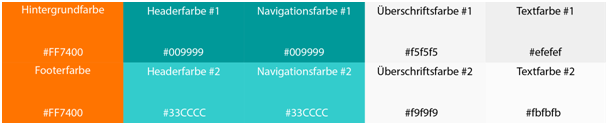
\includegraphics[width=\textwidth]{./img/mini_farb3.png}
\caption{Das 3. alternative Farbschema }
\label{mini_farb3}
\end{figure}

	\subsection{Typographische Gestaltung}

Als Schriftart für Überschriften und die Navigaton wird die Schriftart „Raleway“ verwendet, da diese das Minimalistische im Design unterstreicht. 
Die Schriftgrößen sind möglichst groß gewählt, damit man den Inhalt der Seite sehr gut lesen kann.
\\
Die Schriftfarben sind so gewählt, das diese einen guten Kontrast zum Hintergrund bieten, und dadurch man eine hohe Lesbarkeit erreicht. (siehe Kapitel Farbgebung)


	\subsection{Strukturanalyse der Seite}
Wie in Abbildung \ref{mini_comp3} zu sehen, beinhaltet der Header das Logo mit einem Werbespruch.
Die Navigation sitzt auf der rechten Seite, da diese Seite sich aus der Masse hervorheben soll, denn viele Seiten haben standardmäßig auf der linken Seite oder oben unterhalb des Headers ihre Navigationsleiste. Diese soll ein Drittel des Platzes auf der Webseite einnehmen, damit man die trotzdem sehr schnell erkennen kann. Zudem passt das vom Design her in den goldenen Schnitt. 
\\
Der Content soll zwischen Header und Footer sein, und wird horizontal von der Navigationsleiste eingeschränkt. Dabei soll er bei Textseiten so strukturiert sein, dass bei jedem Abschnitt ein Bild abwechselnd auf der linken und auf der rechten Seite hat. Somit wirkt es trotz des minimalistischem Designs nicht so eintönig. Auf Seiten mit vielen Bildern, zum Beispiel der Seite mit der Produktübersicht, sollen die Elemente tabellarisch und wegen dem Responsive Design auch dynamisch angeordnet sein.
\\
Der Footer enthält Informationen zum Copyright, dem Webseiten-Betreiber sowie ein Link zum Impressum.

\section{Die Würfel sind gefallen}
Nach der Präsentation vor einer Jury ist die Entscheidung gefallen. Ab diesem Zeitpunkt widmet sich die weitere Entwicklung dem innovativen Ansatz. Auch wenn sich einige für die anderen beiden Designs ausgesprochen haben, erhielt er doch den großteil der Stimmen. Es sollte nicht Verwundern, dass ein innovatives Design zu einer innovativen Idee passt.
Trotz des positiven Feedbacks wurde dennoch die Präsentation der einzelnen Artikel im Design bemängelt und es erfolgte der Ratschlag das Kachelsystem des zeitgemäßen Ansatzes in das Ergebnis zu integrieren und weiter zu verfolgen. Die bisherige Formatierung trenne nicht klar genug größere Inhaltsbereiche von untergeordneten Bereichen.
Im weiteren Verlauf dieser Arbeit wird weiter auf die Fusion der einzelnen Ratschläge und Ansätze eingegangen.

\section{Fusion der Ideen}
Zwar wurde der innovative Comp im Plenum als bester Comp gewählt, doch enthalten die anderen Entwürfe Elemente, die übernommen werden sollten. Teile des innovativen Comps, die als „schön“ angesehen wurden, stellten sich später als ziemlich unflexibel und technisch ungünstig dar.
\subsection{Überarbeitung Logo}
\begin{figure} [tp]

\includegraphics[width=\textwidth]{./img/logo3.png}
\caption{Der finale Logo Entwurf}
\label{logo3}
\end{figure}
Aus Rücksicht auf die Wiedererkennbarkeit wurde der Kreis aus dem DigitalHome Logo entfernt (siehe Abbildung \ref{logo3}), da er dem Logo eine kreisförmige Kontur gibt, wodurch diese als wesentliches Wiedererkennungsmerkmal des Logos aufgenommen wird. Das Widererkennungsmerkmal soll jedoch das „Haus“ sein, weshalb diese Form nicht eingerahmt werden darf.

\subsection{Einführung Metro Kacheln}
Nicht nur stellten sich die Produktlinks als unflexibel heraus (Siehe Abschnitt \ref{inno_probs}), sie brechen auch das Layout der Website. Während alle anderen Sections schräge Kanten haben, der Content jedoch in rechteckigen Blöcken organisiert ist, sind jene Links schräge Blöcke, was sie wie eigene Sections aussehen lässt. Die Einführung der Metro Kacheln macht aus den Links Blöcke, die auf Grund ihrer Form korrekterweise einer Section visuell untergeordnet sind und damit genauso zum Content gehören, wie Überschriften und Texte auch. Zusätzlich kommen die Kacheln in unterschiedlichen Größen, dadurch können Hierarchien zwischen den Links gebildet werden, wodurch man Highlights betonen oder weniger wichtige Links in den Hintergrund rücken kann. Und die Kacheln dürfen einen beliebigen Abstand zum rechten Rand der Section haben, ohne das auffällige Stilbrüche auftreten, wodurch das Kachelsystem nochmals flexibler wird.
\subsection{Style Guide}
Nach der Fusion aller Ideen können wir ein einheitliches Branding für DigitalHome festlegen, das wir brauchen, um Entscheidungen zur Gestaltung der Website zu treffen.
\subsection{Menu}
Um schneller navigieren zu können, wurde die Menüleiste mit Symbolen ausgestattet, ohne dass man das Menü öffnen muss und ohne dass der User Text lesen muss. Für eine noch bessere UX auf Desktops muss das Menü nicht mehr durch einen Klick, sondern kann durch hovern der Symbolleiste geöffnet werden. In der Folge kann sich der Nutzer schneller zu anderen Seiten bewegen. Dieses Hover Verhalten gilt nicht nur für die Symbolleiste, das Menü öffnet sich auch bei hovern der Suchleiste. Das macht deshalb Sinn, denn wer etwas auf einer Website sucht, der versucht damit, von der aktuellen Seite auf eine andere zu gelangen, um andere Informationen zu bekommen. Vielleicht wurde das Menü auch gar nicht oder nicht als solches wahrgenommen. Eine gute Gelegenheit, dem Nutzer zu zeigen, wie er navigieren kann. Findet er keinen passenden Link, kann er trotzdem die Suchleiste benutzen.

\section{Ableiten von Unterseiten}

\section{Optimierung}
Die Webseite war aber trotz allem noch lange nicht perfekt. 
\\
\\
Der CSS- und Javascript-Quelltext wurde modularisiert, sodass man eine einfachere Wartung und Optimierung machen kann.
\\
\\
Die Bilder waren zu groß, so dass es Probleme mit Transition-Effekten gab, da der Browser mit dem Rendern nicht nachkam. Dies wurde durch Komprimieren mit Hilfe von Minifyern behoben, worauf jetzt noch genauer eingegangen wird.
\\
Damit der Quelltext für den Browser schneller und einfacher zu interpretieren ist, wurden im Anschluss Programme verwendet, sogenannte Minifyer, die alle für den Browser unnötige Zeichen, wie Kommentare oder Leerzeichen aus dem Quelltext entfernen und somit die komprimiert und für den Computer vereinfacht. Mit Hilfe dieser Programme wurden Bilder, HTML, CSS, und JavaScript-Dateien komprimiert. Da aber der Quelltext zwar für den Computer viel einfacher und schneller lesbar ist, ist es für Menschen nicht mehr so einfach lesbar. Deswegen wurde ein Source-Verzeichnis angelegt, worin gearbeitet wird, und im Anschluss die Minifyer die eigentlichen Quelltext-Dateien, worauf sich der Browser bezieht, verkleinert. 
\\
\\
Das zuvor implementierte Canvas wurde wieder aus der Startseite herausgenommen, da dieses zu große Probleme beim Laden der Seite bereitet hat. Da aber das Konzept des Canvas gefallen hatte, wurde es als Hintergrundeffekt der Fehler- und der Wartungsseiten eingesetzt. Darauf wird in Kapitel \ref{descr_canvas} genauer eingegangen.
